%!TEX program = xelatex
\documentclass[11pt,article,oneside]{memoir}
\usepackage{org-preamble-xelatex}
\DisemulatePackage{setspace}
\usepackage{setspace}
% \input{vc}

\usepackage{longtable}

\usepackage{graphicx}
% We will generate all images so they have a width \maxwidth. This means
% that they will get their normal width if they fit onto the page, but
% are scaled down if they would overflow the margins.
\makeatletter
\def\maxwidth{\ifdim\Gin@nat@width>\linewidth\linewidth
\else\Gin@nat@width\fi}
\makeatother
\let\Oldincludegraphics\includegraphics
\renewcommand{\includegraphics}[1]{\Oldincludegraphics[width=\maxwidth]{#1}}

\title{\bigskip \bigskip How Does the State Speak of Globalisation? A Quantitative Text-Mining
Approach}

%\author{}

\author{\Large Justin Murphy\vspace{0.05in} \newline\normalsize\emph{University of Southampton} \newline\footnotesize \url{j.murphy@soton.ac.uk}\vspace*{0.2in}\newline }

%\author{Justin Murphy (University of Southampton)}

\date{}


\begin{document}  
\setkeys{Gin}{width=1\textwidth} 	
\setromanfont[Mapping=tex-text,Numbers=OldStyle]{Georgia} 
\setsansfont[Mapping=tex-text]{Gill Sans} 
\setmonofont[Mapping=tex-text,Scale=0.8]{Consolas}
\chapterstyle{article-2}

\doublespacing


\maketitle



\begin{abstract}

\noindent Scholars argue that globalisation is strategically deployed by
governments (Hay and Rosamond 2011). This article is the first
large-scale quantitative assessment of this argument, using text-mining
and machine learning techniques to analyze how the government of the
United Kingdom has deployed the term `globalisation.' Specifically, this
article exploits the newly released United Kingdom Government Web
Archive to analyze a random sample of more than 60,000 web pages
published across the entire UK government web system.

\end{abstract}


I requested 150,000 web pages, received 67k and about 1k were errors.
Thus, the final sample consists of a corpus of dtm

\pagebreak

\subsubsection{Descriptive Statistics}\label{descriptive-statistics}

\begin{figure}[htbp]
\centering
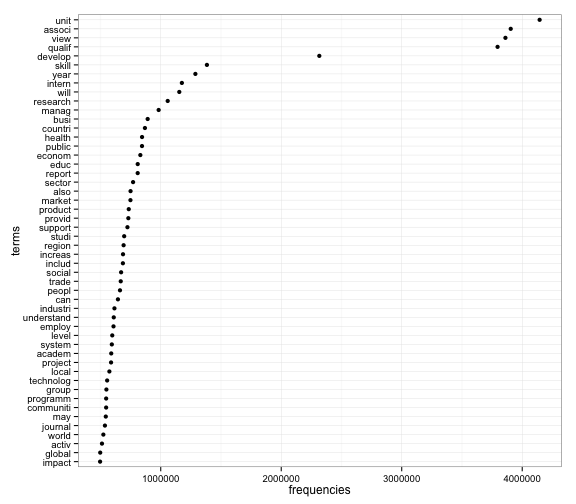
\includegraphics{figure/globalisation_frequency_plot.png}
\caption{Most frequent terms}
\end{figure}

\pagebreak

\paragraph{Correlated terms}\label{correlated-terms}

\begin{longtable}[c]{@{}cc@{}}
\toprule\addlinespace
\begin{minipage}[b]{0.13\columnwidth}\centering
Terms
\end{minipage} & \begin{minipage}[b]{0.13\columnwidth}\centering
Globalis
\end{minipage}
\\\addlinespace
\midrule\endhead
\begin{minipage}[t]{0.13\columnwidth}\centering
vision
\end{minipage} & \begin{minipage}[t]{0.13\columnwidth}\centering
0.9
\end{minipage}
\\\addlinespace
\begin{minipage}[t]{0.13\columnwidth}\centering
emphasi
\end{minipage} & \begin{minipage}[t]{0.13\columnwidth}\centering
0.87
\end{minipage}
\\\addlinespace
\begin{minipage}[t]{0.13\columnwidth}\centering
secondari
\end{minipage} & \begin{minipage}[t]{0.13\columnwidth}\centering
0.84
\end{minipage}
\\\addlinespace
\begin{minipage}[t]{0.13\columnwidth}\centering
context
\end{minipage} & \begin{minipage}[t]{0.13\columnwidth}\centering
0.83
\end{minipage}
\\\addlinespace
\begin{minipage}[t]{0.13\columnwidth}\centering
legaci
\end{minipage} & \begin{minipage}[t]{0.13\columnwidth}\centering
0.82
\end{minipage}
\\\addlinespace
\begin{minipage}[t]{0.13\columnwidth}\centering
implic
\end{minipage} & \begin{minipage}[t]{0.13\columnwidth}\centering
0.81
\end{minipage}
\\\addlinespace
\begin{minipage}[t]{0.13\columnwidth}\centering
amongst
\end{minipage} & \begin{minipage}[t]{0.13\columnwidth}\centering
0.8
\end{minipage}
\\\addlinespace
\begin{minipage}[t]{0.13\columnwidth}\centering
educ
\end{minipage} & \begin{minipage}[t]{0.13\columnwidth}\centering
0.79
\end{minipage}
\\\addlinespace
\begin{minipage}[t]{0.13\columnwidth}\centering
vocat
\end{minipage} & \begin{minipage}[t]{0.13\columnwidth}\centering
0.78
\end{minipage}
\\\addlinespace
\begin{minipage}[t]{0.13\columnwidth}\centering
perceiv
\end{minipage} & \begin{minipage}[t]{0.13\columnwidth}\centering
0.76
\end{minipage}
\\\addlinespace
\bottomrule
\end{longtable}

\pagebreak

\section{Cluster analysis}\label{cluster-analysis}

\begin{verbatim}
## [1] Cluster 1      
##  [1] will      report    can       committe  increas   level     offic    
##  [8] also      school    need      invest    busi      includ    compani  
## [15] govern    transport use       industri  number    respons  
## [1] Cluster 2      
##  [1] journal   intern    manag     technolog system    engin     comput   
##  [8] titl      publish   onlin     euro      print     intellig  busi     
## [15] innov     enterpris electron  scienc    sustain   price    
## [1] Cluster 3      
##  [1] health   public   care     journal  nhs      diseas   find    
##  [8] polici   author   avail    articl   sourc    impact   london  
## [15] research exclud   refin    similar  add      clinic  
## [1] Cluster 4      
##  [1] research  skip      accesskey esrc      social    search    page     
##  [8] studi     public    econom    news      scienc    impact    societi  
## [15] contact   output    fund      grant     guidanc   work     
## [1] Cluster 5      
##  [1] eldi      websit    globalis  topic     home      develop   countri  
##  [8] inform    guid      what      announc   profil    publish   site     
## [15] job       map       event     communiti visit     new      
## [1] Cluster 6      
##  [1] unit       qualif     associ     view       understand skill     
##  [7] provid     design     introduct  perform    listen     write     
## [13] sport      leisur     treatment  music      physic     read      
## [19] techniqu   wale      
## [1] Cluster 7      
##  [1] eldi       group      develop    space      communiti  member    
##  [7] interest   friend     help       blog       search     opinion   
## [13] profil     home       comment    livelihood famili     secur     
## [19] name       aid       
## [1] Cluster 8      
##  [1] oper     countri  procur   organis  non      specif   servic  
##  [8] tel      profit   project  search   india    result   programm
## [15] africa   support  govern   china    fund     aid     
## [1] Cluster 9      
##  [1] academ    year      breakdown geograph  coverag   articl    region   
##  [8] pdf       labour    econom    market    review    countri   statist  
## [15] filter    economi   trend     releas    book      sep      
## [1] "Cluster Membership"
## 
##     1     2     3     4     5     6     7     8     9 
## 46337   907  2235  5459  3535  2345  2121   779  2696 
## [1] "Within cluster sum of squares by cluster"
## [1] 383.976905   0.009232  18.591247  36.403308  28.291523   4.239123
## [7]  14.269600  21.928006  55.741371
\end{verbatim}

\pagebreak

\section{Appendix}\label{appendix}

This is the appendix.

\begin{figure}[htbp]
\centering
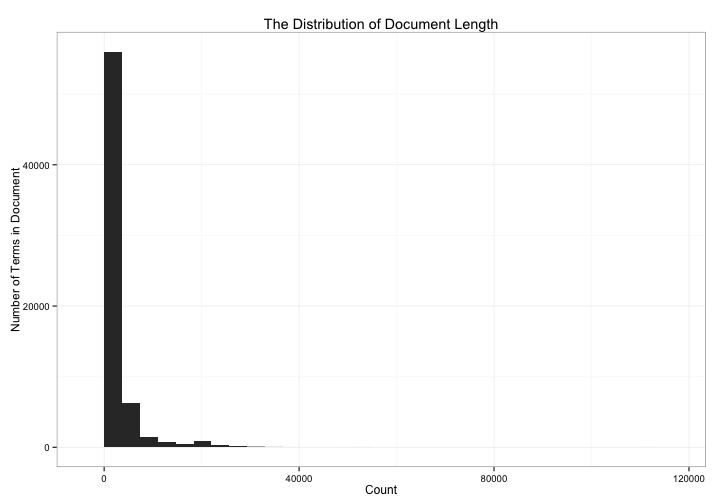
\includegraphics{figure/Document-Lengths.png}
\caption{Document lengths}
\end{figure}

\begin{verbatim}
##              Length Class  Mode   
## cluster      66414  -none- numeric
## centers      17640  -none- numeric
## totss            1  -none- numeric
## withinss         9  -none- numeric
## tot.withinss     1  -none- numeric
## betweenss        1  -none- numeric
## size             9  -none- numeric
## iter             1  -none- numeric
## ifault           1  -none- numeric
\end{verbatim}

\begin{figure}[htbp]
\centering
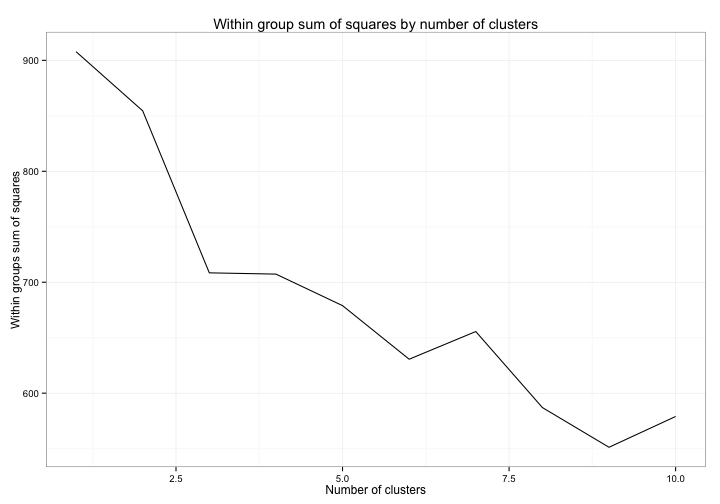
\includegraphics{figure/Cluster-Diagnostics.png}
\caption{Binwidth}
\end{figure}

\begin{verbatim}
##       Topic 1    Topic 2     Topic 3        Topic 4    Topic 5   
##  [1,] "skill"    "school"    "globalis"     "financi"  "product" 
##  [2,] "develop"  "use"       "websit"       "market"   "per"     
##  [3,] "educ"     "educ"      "global"       "intern"   "year"    
##  [4,] "globalis" "teacher"   "eldi"         "globalis" "countri" 
##  [5,] "countri"  "ict"       "polici"       "capit"    "price"   
##  [6,] "dfid"     "can"       "new"          "bank"     "world"   
##  [7,] "also"     "learn"     "home"         "develop"  "cost"    
##  [8,] "train"    "dfid"      "unit"         "economi"  "market"  
##  [9,] "sector"   "project"   "europ"        "global"   "industri"
## [10,] "research" "student"   "relationship" "econom"   "export"  
## [11,] "need"     "technolog" "intern"       "risk"     "increas" 
## [12,] "cultur"   "peopl"     "busi"         "countri"  "trade"   
## [13,] "nation"   "work"      "inform"       "increas"  "cent"    
## [14,] "econom"   "communiti" "trade"        "growth"   "import"  
## [15,] "world"    "activ"     "countri"      "system"   "develop" 
## [16,] "global"   "experi"    "world"        "will"     "govern"  
## [17,] "poverti"  "comput"    "state"        "polici"   "period"  
## [18,] "women"    "develop"   "tel"          "servic"   "even"    
## [19,] "increas"  "also"      "work"         "benefit"  "exchang" 
## [20,] "privat"   "teach"     "secur"        "invest"   "howev"   
##       Topic 6    Topic 7    Topic 8    Topic 9     
##  [1,] "pay"      "develop"  "develop"  "develop"   
##  [2,] "plus"     "relat"    "countri"  "impact"    
##  [3,] "fair"     "skill"    "trade"    "research"  
##  [4,] "intern"   "strategi" "intern"   "agricultur"
##  [5,] "institut" "level"    "govern"   "increas"   
##  [6,] "concern"  "govern"   "work"     "servic"    
##  [7,] "commerc"  "globalis" "will"     "report"    
##  [8,] "encourag" "countri"  "polici"   "product"   
##  [9,] "certain"  "term"     "world"    "rural"     
## [10,] "popul"    "polici"   "peopl"    "food"      
## [11,] "import"   "nation"   "import"   "use"       
## [12,] "cent"     "market"   "poverti"  "also"      
## [13,] "constitu" "requir"   "poor"     "may"       
## [14,] "assur"    "key"      "globalis" "health"    
## [15,] "programm" "global"   "effect"   "popul"     
## [16,] "public"   "educ"     "invest"   "water"     
## [17,] "accord"   "two"      "price"    "migrat"    
## [18,] "social"   "differ"   "inflat"   "area"      
## [19,] "parti"    "state"    "can"      "growth"    
## [20,] "term"     "competit" "increas"  "poverti"
\end{verbatim}

\pagebreak

\section{References}\label{references}

\setlength{\parindent}{-0.2in} \setlength{\leftskip}{0.2in}
\setlength{\parskip}{8pt} \vspace*{-0.2in} \noindent

Hay, Colin, and Ben Rosamond. 2011. ``Globalization, European
Integration and the Discursive Construction of Economic Imperatives.''
\emph{dx.doi.org.libproxy.temple.edu} 9(2): 147--67.
\url{http://www.tandfonline.com/doi/abs/10.1080/13501760110120192}.


\end{document}